% !TEX TS-program = pdflatex
\documentclass[11pt]{article}

% -------------------- Packages --------------------
\usepackage[a4paper,margin=1in]{geometry}
\usepackage{amsmath,amssymb}
\usepackage[T1]{fontenc}
\usepackage{lmodern}
\usepackage{xcolor}
\usepackage{tcolorbox}
\tcbuselibrary{skins,breakable}
\usepackage{enumitem}
\usepackage{hyperref}
\usepackage{tikz}
\usetikzlibrary{calc,angles,quotes,arrows.meta}

\pagestyle{empty}

% -------------------- Dark Theme Colors --------------------
\definecolor{bg}{HTML}{000000}
\definecolor{pairbg}{HTML}{121212}
\definecolor{solbg}{HTML}{0A0A0A}
\definecolor{border}{HTML}{2A2A2A}
\definecolor{text}{HTML}{FFFFFF}
\definecolor{muted}{HTML}{C9CDD3}
\definecolor{gold}{HTML}{FFD700}
\definecolor{green}{HTML}{4ADE80}
\definecolor{cyan}{HTML}{38BDF8}

\pagecolor{bg}
\color{text}

\hypersetup{
  colorlinks=true,
  linkcolor=cyan,
  urlcolor=cyan
}

\setlength{\parindent}{0pt}
\setlength{\parskip}{10pt}

% Help LaTeX avoid overfull lines globally
\sloppy
\setlength{\emergencystretch}{3em}

\setlist[itemize]{left=1.4em,itemsep=6pt,topsep=6pt}
\setlist[enumerate]{left=1.6em,itemsep=4pt,topsep=4pt}

% -------------------- tcolorbox Base --------------------
\tcbset{
  enhanced,
  breakable,
  arc=12pt,
  boxrule=0.8pt,
  left=14pt,right=14pt,top=12pt,bottom=12pt
}

\newtcolorbox{QAPair}[1]{%
  colback=pairbg,
  colbacklower=solbg,
  colframe=border,
  coltext=text,
  title=\textcolor{gold}{\bfseries #1},
  fonttitle=\bfseries,
  coltitle=text,
  segmentation style={draw=border, dashed, line width=0.6pt},
  before upper=\raggedright,
  before lower=\raggedright
}

\newtcolorbox{QuickBox}{%
  colback=pairbg,
  colframe=cyan,
  coltext=text,
  fontupper=\color{text}\raggedright,
  borderline north={4pt}{0pt}{cyan},
  arc=14pt,
  boxrule=0.8pt
}

% Helper for step headings
\newcommand{\Step}[1]{\textcolor{muted}{\textbf{Step #1:}}}

% Small centered diagram block
\newenvironment{StepDiagram}{\par\medskip\begin{center}}{\end{center}\medskip}

% TikZ styles
\tikzset{
  base/.style={draw=text, line width=0.9pt, line cap=round, line join=round},
  new/.style={draw=cyan, line width=1.2pt, line cap=round, line join=round},
  help/.style={draw=muted, dashed, line width=0.9pt},
  ang/.style={draw=gold, line width=1.0pt},
  dot/.style={circle, fill=text, inner sep=1.2pt},
  lab/.style={text=text, font=\small},
  labm/.style={text=muted, font=\small},
}

% Small "equation diagram" box
\newcommand{\EqDiagram}[1]{%
\begin{StepDiagram}
\begin{tikzpicture}
\node[draw=border, rounded corners=10pt, inner sep=8pt, text=text, align=left, text width=0.88\linewidth] {#1};
\end{tikzpicture}
\end{StepDiagram}
}

% ============================================================
\begin{document}

\begin{center}
{\LARGE\bfseries \textcolor{gold}{Exercise 9.3 --- Solutions}}\\[-2pt]
\end{center}

% -------------------- Quick formulas + clean diagrams --------------------
\begin{QuickBox}
{\color{cyan}\bfseries Quick formulas (Chords, arcs, and angles)}\par\medskip

\begin{itemize}
\item \textbf{Equal chords $\Longleftrightarrow$ equal arcs $\Longleftrightarrow$ equal central angles.}
\begin{StepDiagram}
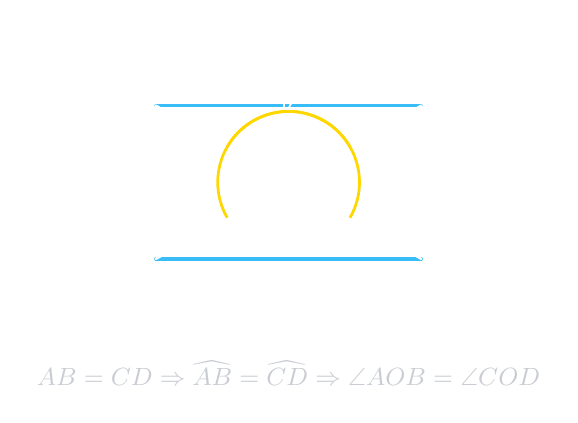
\begin{tikzpicture}[scale=0.95]
  \def\r{2.05}
  \coordinate (O) at (0,0);
  \coordinate (A) at ({\r*cos(150)},{\r*sin(150)});
  \coordinate (B) at ({\r*cos( 30)},{\r*sin( 30)});
  \coordinate (C) at ({\r*cos(210)},{\r*sin(210)});
  \coordinate (D) at ({\r*cos(330)},{\r*sin(330)});

  \draw[base] (O) circle (\r);
  \node[dot,label={[lab]below:$O$}] at (O) {};

  \draw[new] (A)--(B);
  \draw[new] (C)--(D);

  \draw[base] (O)--(A) (O)--(B);
  \draw[base] (O)--(C) (O)--(D);

  \pic[ang,"$\theta$",lab,angle radius=9mm,angle eccentricity=1.15] {angle=B--O--A};
  \pic[ang,"$\theta$",lab,angle radius=9mm,angle eccentricity=1.15] {angle=D--O--C};

  \node[labm] at (0,-2.55) {$AB=CD \Rightarrow \widehat{AB}=\widehat{CD} \Rightarrow \angle AOB=\angle COD$};
\end{tikzpicture}
\end{StepDiagram}

\item \textbf{Inscribed angle theorem:} angle at circumference $=$ half the angle at centre (same arc).
\[
\angle ACB = \tfrac12\,\angle AOB.
\]
\begin{StepDiagram}
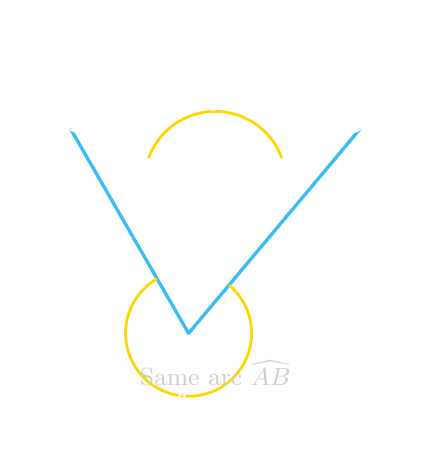
\begin{tikzpicture}[scale=0.95]
  \def\r{2.05}
  \coordinate (O) at (0,0);
  \coordinate (A) at ({\r*cos(160)},{\r*sin(160)});
  \coordinate (B) at ({\r*cos( 20)},{\r*sin( 20)});
  \coordinate (C) at ({\r*cos(260)},{\r*sin(260)});

  \draw[base] (O) circle (\r);
  \node[dot,label={[lab]below:$O$}] at (O) {};
  \node[dot,label={[lab]left:$A$}] at (A) {};
  \node[dot,label={[lab]right:$B$}] at (B) {};
  \node[dot,label={[lab]below:$C$}] at (C) {};

  \draw[new] (A)--(C) (B)--(C);
  \draw[base] (O)--(A) (O)--(B);
  \draw[base] (A)--(B);

  \pic[ang,"$\theta$",lab,angle radius=9mm,angle eccentricity=1.12] {angle=B--O--A};
  \pic[ang,"$\tfrac{\theta}{2}$",lab,angle radius=8mm,angle eccentricity=1.15] {angle=A--C--B};

  \node[labm] at (0,-2.55) {Same arc $\widehat{AB}$};
\end{tikzpicture}
\end{StepDiagram}

\item \textbf{Arc length:} for the same circle, $\displaystyle s \propto \theta$ (so $\frac{s_1}{s_2}=\frac{\theta_1}{\theta_2}$).
\[
s=\frac{\theta}{360^\circ}\,(2\pi r)\quad (\theta \text{ in degrees}).
\]
\begin{StepDiagram}
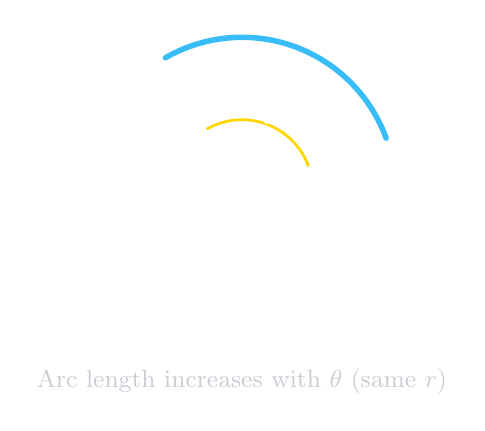
\begin{tikzpicture}[scale=0.95]
  \def\r{2.05}
  \coordinate (O) at (0,0);
  \coordinate (A) at ({\r*cos(120)},{\r*sin(120)});
  \coordinate (B) at ({\r*cos( 20)},{\r*sin( 20)});

  \draw[base] (O) circle (\r);
  \node[dot,label={[lab]below:$O$}] at (O) {};
  \draw[base] (O)--(A) (O)--(B);
  \draw[new, line width=2pt] (A) arc[start angle=120,end angle=20,radius=\r];

  \pic[ang,"$\theta$",lab,angle radius=9mm,angle eccentricity=1.12] {angle=B--O--A};
  \node[labm] at (0,-2.55) {Arc length increases with $\theta$ (same $r$)};
\end{tikzpicture}
\end{StepDiagram}
\end{itemize}
\end{QuickBox}

% ============================================================
% Q1(i)
\begin{QAPair}{Question 1 (i)}
\textcolor{gold}{\bfseries Question:} In the figure, chord $AB=$ chord $BC$. Is $\widehat{AB}=\widehat{BC}$?
\tcblower
\textcolor{green}{\bfseries Answer:}\par

\Step{1} Draw the circle with centre $P$ and mark equal chords $AB$ and $BC$.
\begin{StepDiagram}
\begin{tikzpicture}[scale=0.95]
  \def\r{2.1}
  \coordinate (P) at (0,0);
  \coordinate (A) at ({\r*cos(150)},{\r*sin(150)});
  \coordinate (B) at ({\r*cos(210)},{\r*sin(210)});
  \coordinate (C) at ({\r*cos(270)},{\r*sin(270)});
  \draw[base] (P) circle (\r);
  \node[dot,label={[lab]right:$P$}] at (P) {};
  \node[dot,label={[lab]left:$A$}] at (A) {};
  \node[dot,label={[lab]below left:$B$}] at (B) {};
  \node[dot,label={[lab]below:$C$}] at (C) {};
  \draw[new] (A)--(B);
  \draw[new] (B)--(C);
\end{tikzpicture}
\end{StepDiagram}

\Step{2} \textbf{Equal chords subtend equal arcs} in the same circle.
\EqDiagram{$AB=BC \;\Rightarrow\; \widehat{AB}=\widehat{BC}.$}

\[
\boxed{\widehat{AB}=\widehat{BC}}
\]
\end{QAPair}

% Q1(ii)
\begin{QAPair}{Question 1 (ii)}
\textcolor{gold}{\bfseries Question:} Is $\angle APB=\angle BPC$?
\tcblower
\textcolor{green}{\bfseries Answer:}\par

\Step{1} Join $PA,PB,PC$ (radii).
\begin{StepDiagram}
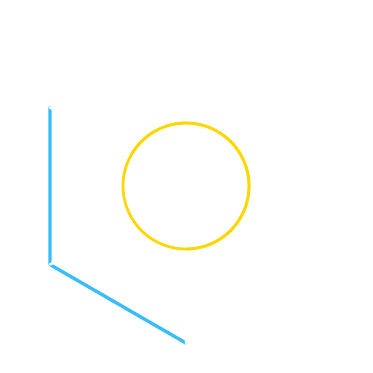
\begin{tikzpicture}[scale=0.95]
  \def\r{2.1}
  \coordinate (P) at (0,0);
  \coordinate (A) at ({\r*cos(150)},{\r*sin(150)});
  \coordinate (B) at ({\r*cos(210)},{\r*sin(210)});
  \coordinate (C) at ({\r*cos(270)},{\r*sin(270)});
  \draw[base] (P) circle (\r);
  \node[dot,label={[lab]right:$P$}] at (P) {};
  \draw[new] (A)--(B) (B)--(C);
  \draw[base] (P)--(A) (P)--(B) (P)--(C);
  \pic[ang,"$\theta$",lab,angle radius=8mm,angle eccentricity=1.15] {angle=B--P--A};
  \pic[ang,"$\theta$",lab,angle radius=8mm,angle eccentricity=1.15] {angle=C--P--B};
\end{tikzpicture}
\end{StepDiagram}

\Step{2} Equal chords $\Rightarrow$ equal arcs $\Rightarrow$ equal central angles.
\EqDiagram{$AB=BC \Rightarrow \angle APB=\angle BPC.$}

\[
\boxed{\angle APB=\angle BPC}
\]
\end{QAPair}

% Q1(iii)
\begin{QAPair}{Question 1 (iii)}
\textcolor{gold}{\bfseries Question:} If $\widehat{AB}<\widehat{AD}$, what is the relation between the corresponding chords?
\tcblower
\textcolor{green}{\bfseries Answer:}\par

\Step{1} Bigger arc $\Rightarrow$ bigger central angle.
\begin{StepDiagram}
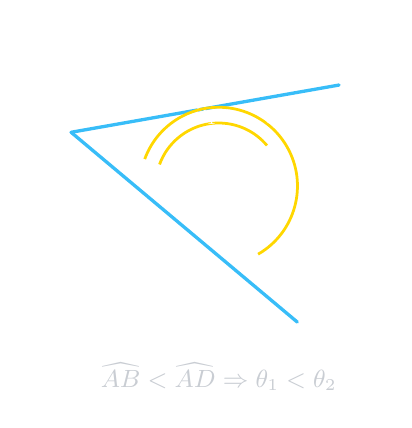
\begin{tikzpicture}[scale=0.95]
  \def\r{2.1}
  \coordinate (P) at (0,0);
  \coordinate (A) at ({\r*cos(160)},{\r*sin(160)});
  \coordinate (B) at ({\r*cos( 40)},{\r*sin( 40)});
  \coordinate (D) at ({\r*cos(300)},{\r*sin(300)});
  \draw[base] (P) circle (\r);
  \node[dot,label={[lab]below:$P$}] at (P) {};
  \node[dot,label={[lab]left:$A$}] at (A) {};
  \node[dot,label={[lab]right:$B$}] at (B) {};
  \node[dot,label={[lab]below right:$D$}] at (D) {};
  \draw[base] (P)--(A) (P)--(B) (P)--(D);
  \draw[new] (A)--(B);
  \draw[new] (A)--(D);
  \pic[ang,"$\theta_1$",lab,angle radius=8mm,angle eccentricity=1.15] {angle=B--P--A};
  \pic[ang,"$\theta_2$",lab,angle radius=10mm,angle eccentricity=1.15] {angle=D--P--A};
  \node[labm] at (0,-2.55) {$\widehat{AB}<\widehat{AD}\Rightarrow \theta_1<\theta_2$};
\end{tikzpicture}
\end{StepDiagram}

\Step{2} Bigger central angle $\Rightarrow$ bigger chord (same circle).
\EqDiagram{$\widehat{AB}<\widehat{AD}\Rightarrow AB<AD.$}

\[
\boxed{AB<AD}
\]
\end{QAPair}

% ============================================================
% Q2
\begin{QAPair}{Question 2}
\textcolor{gold}{\bfseries Question:} In the figure, $\widehat{AC}=\widehat{BD}$. Prove that $AB\parallel CD$.
\tcblower
\textcolor{green}{\bfseries Answer:}\par

\Step{1} Join the chord $BC$ (use it as a transversal).
\begin{StepDiagram}
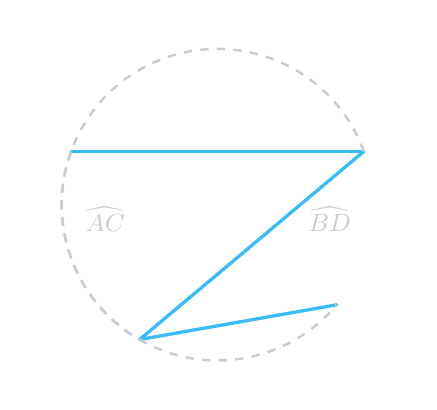
\begin{tikzpicture}[scale=0.92]
  \def\r{2.15}
  \coordinate (O) at (0,0);
  \coordinate (A) at ({\r*cos(160)},{\r*sin(160)});
  \coordinate (B) at ({\r*cos( 20)},{\r*sin( 20)});
  \coordinate (C) at ({\r*cos(240)},{\r*sin(240)});
  \coordinate (D) at ({\r*cos(320)},{\r*sin(320)});

  \draw[base] (O) circle (\r);
  \node[dot,label={[lab]below:$O$}] at (O) {};
  \node[dot,label={[lab]left:$A$}] at (A) {};
  \node[dot,label={[lab]right:$B$}] at (B) {};
  \node[dot,label={[lab]below left:$C$}] at (C) {};
  \node[dot,label={[lab]below right:$D$}] at (D) {};

  \draw[new] (A)--(B);
  \draw[new] (C)--(D);
  \draw[new] (B)--(C);

  % light arc hints (visual only)
  \draw[help] (A) arc[start angle=160,end angle=240,radius=\r];
  \draw[help] (B) arc[start angle=20,end angle=320,radius=\r];
  \node[labm] at (-1.55,-0.2) {$\widehat{AC}$};
  \node[labm] at ( 1.55,-0.2) {$\widehat{BD}$};
\end{tikzpicture}
\end{StepDiagram}

\Step{2} By the inscribed-angle theorem,
\[
\angle ABC=\tfrac12\,\widehat{AC},
\qquad
\angle BCD=\tfrac12\,\widehat{BD}.
\]
\EqDiagram{$\widehat{AC}=\widehat{BD}\Rightarrow \angle ABC=\angle BCD.$}

\Step{3} Since $\angle ABC=\angle BCD$ are alternate interior angles with transversal $BC$,
\[
AB\parallel CD.
\]
\begin{StepDiagram}
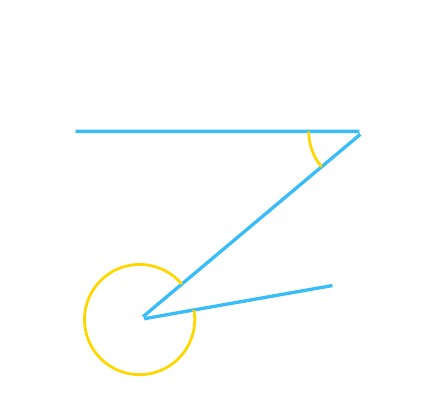
\begin{tikzpicture}[scale=0.92]
  \def\r{2.15}
  \coordinate (A) at ({\r*cos(160)},{\r*sin(160)});
  \coordinate (B) at ({\r*cos( 20)},{\r*sin( 20)});
  \coordinate (C) at ({\r*cos(240)},{\r*sin(240)});
  \coordinate (D) at ({\r*cos(320)},{\r*sin(320)});
  \coordinate (O) at (0,0);

  \draw[base] (O) circle (\r);
  \draw[new] (A)--(B) (C)--(D) (B)--(C);
  \node[dot,label={[lab]left:$A$}] at (A) {};
  \node[dot,label={[lab]right:$B$}] at (B) {};
  \node[dot,label={[lab]below left:$C$}] at (C) {};
  \node[dot,label={[lab]below right:$D$}] at (D) {};

  \pic[ang,"$\alpha$",lab,angle radius=7mm,angle eccentricity=1.2] {angle=A--B--C};
  \pic[ang,"$\alpha$",lab,angle radius=7mm,angle eccentricity=1.2] {angle=B--C--D};
\end{tikzpicture}
\end{StepDiagram}

\[
\boxed{AB\parallel CD}
\]
\end{QAPair}

% ============================================================
% Q3
\begin{QAPair}{Question 3}
\textcolor{gold}{\bfseries Question:} Chords $AB$ and $CD$ intersect at $P$. If $AB=CD$, prove that $\widehat{AB}=\widehat{CD}$.
\tcblower
\textcolor{green}{\bfseries Answer:}\par

\Step{1} Mark equal chords $AB$ and $CD$ in the same circle.
\begin{StepDiagram}
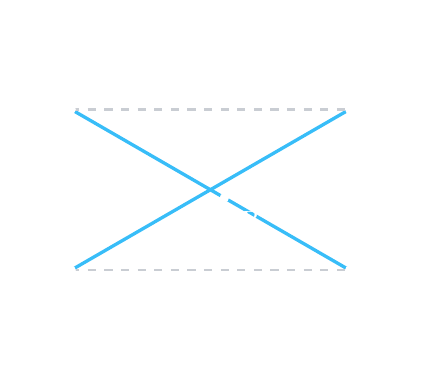
\begin{tikzpicture}[scale=0.95]
  \def\r{2.15}
  \coordinate (O) at (0,0);
  \coordinate (A) at ({\r*cos(150)},{\r*sin(150)});
  \coordinate (B) at ({\r*cos(330)},{\r*sin(330)});
  \coordinate (C) at ({\r*cos(210)},{\r*sin(210)});
  \coordinate (D) at ({\r*cos( 30)},{\r*sin( 30)});
  \coordinate (P) at ($(A)!0.55!(B)$);

  \draw[base] (O) circle (\r);
  \node[dot,label={[lab]below:$O$}] at (O) {};

  \draw[new] (A)--(B);
  \draw[new] (C)--(D);

  \draw[help] (A)--(D);
  \draw[help] (C)--(B);

  \node[dot,label={[lab]below right:$P$}] at (P) {};
  \node[dot,label={[lab]left:$A$}] at (A) {};
  \node[dot,label={[lab]right:$B$}] at (B) {};
  \node[dot,label={[lab]below left:$C$}] at (C) {};
  \node[dot,label={[lab]above right:$D$}] at (D) {};
\end{tikzpicture}
\end{StepDiagram}

\Step{2} In a circle, \textbf{equal chords subtend equal arcs}.
\EqDiagram{$AB=CD \;\Rightarrow\; \widehat{AB}=\widehat{CD}.$}

\[
\boxed{\widehat{AB}=\widehat{CD}}
\]
\end{QAPair}

% ============================================================
% Q4(i)
\begin{QAPair}{Question 4 (i)}
\textcolor{gold}{\bfseries Question:} Two circles have radii $2$ cm and $4$ cm (centres $P$ and $Q$). Arcs $\widehat{AB}$ and $\widehat{CD}$ satisfy $\angle APB=\angle CQD$. Are the arcs congruent?
\tcblower
\textcolor{green}{\bfseries Answer:}\par

\Step{1} Same central angle, different radii.
\begin{StepDiagram}
\begin{tikzpicture}[scale=0.92]
  \def\rA{1.4}
  \def\rB{2.4}
  \coordinate (P) at (-2.6,0);
  \coordinate (Q) at ( 2.6,0);

  \coordinate (A) at ($(P)+({\rA*cos(130)},{\rA*sin(130)})$);
  \coordinate (B) at ($(P)+({\rA*cos( 20)},{\rA*sin( 20)})$);

  \coordinate (C) at ($(Q)+({\rB*cos(130)},{\rB*sin(130)})$);
  \coordinate (D) at ($(Q)+({\rB*cos( 20)},{\rB*sin( 20)})$);

  \draw[base] (P) circle (\rA);
  \draw[base] (Q) circle (\rB);
  \node[dot,label={[lab]below:$P$}] at (P) {};
  \node[dot,label={[lab]below:$Q$}] at (Q) {};

  \draw[base] (P)--(A) (P)--(B);
  \draw[base] (Q)--(C) (Q)--(D);

  \draw[new, line width=2pt] (A) arc[start angle=130,end angle=20,radius=\rA];
  \draw[new, line width=2pt] (C) arc[start angle=130,end angle=20,radius=\rB];

  \pic[ang,"$\theta$",lab,angle radius=7mm,angle eccentricity=1.1] {angle=B--P--A};
  \pic[ang,"$\theta$",lab,angle radius=10mm,angle eccentricity=1.1] {angle=D--Q--C};

  \node[lab] at (-2.6,-1.85) {$r=2$};
  \node[lab] at ( 2.6,-2.55) {$r=4$};
\end{tikzpicture}
\end{StepDiagram}

\Step{2} Arc length $s=\dfrac{\theta}{360^\circ}(2\pi r)$ depends on $r$.
So with the same $\theta$ but different $r$, arc lengths differ.
\EqDiagram{Same $\theta$, but $r$ different $\Rightarrow$ arc lengths different $\Rightarrow$ arcs are \emph{not} congruent.}

\[
\boxed{\text{No, the arcs are not congruent.}}
\]
\end{QAPair}

% Q4(ii)
\begin{QAPair}{Question 4 (ii)}
\textcolor{gold}{\bfseries Question:} What is the relation between the lengths of arcs $\widehat{AB}$ and $\widehat{CD}$?
\tcblower
\textcolor{green}{\bfseries Answer:}\par

\Step{1} For the same central angle $\theta$, arc length is proportional to radius:
\[
s=r\theta \quad (\theta\text{ in radians}) \;\Rightarrow\; \frac{s_1}{s_2}=\frac{r_1}{r_2}.
\]
\EqDiagram{$\displaystyle \frac{\text{len}(\widehat{AB})}{\text{len}(\widehat{CD})}=\frac{2}{4}=\frac{1}{2}.$}

\Step{2} Hence,
\[
\text{len}(\widehat{CD}) = 2\,\text{len}(\widehat{AB}).
\]
\begin{StepDiagram}
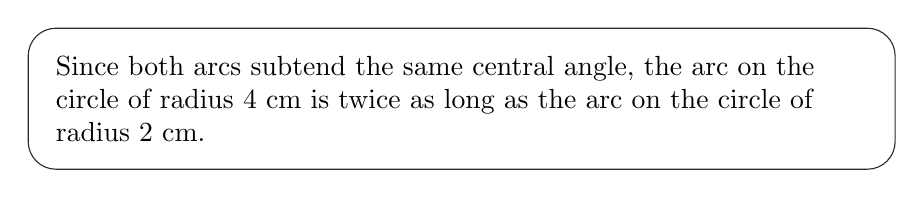
\begin{tikzpicture}[scale=0.92]
  \node[draw=border, rounded corners=10pt, inner sep=10pt, align=left, text width=0.85\linewidth]{
  Since both arcs subtend the same central angle, the arc on the circle of radius $4$ cm is twice as long as the arc on the circle of radius $2$ cm.};
\end{tikzpicture}
\end{StepDiagram}

\[
\boxed{\text{len}(\widehat{CD}) : \text{len}(\widehat{AB}) = 2:1}
\]
\end{QAPair}

% Q4(iii)
\begin{QAPair}{Question 4 (iii)}
\textcolor{gold}{\bfseries Question:} Show that $\triangle APB \sim \triangle CQD$.
\tcblower
\textcolor{green}{\bfseries Answer:}\par

\Step{1} Radii give proportional sides:
\[
AP=BP=2,\qquad CQ=QD=4.
\]
\begin{StepDiagram}
\begin{tikzpicture}[scale=0.92]
  \def\rA{1.4}
  \def\rB{2.4}
  \coordinate (P) at (-2.6,0);
  \coordinate (Q) at ( 2.6,0);

  \coordinate (A) at ($(P)+({\rA*cos(130)},{\rA*sin(130)})$);
  \coordinate (B) at ($(P)+({\rA*cos( 20)},{\rA*sin( 20)})$);

  \coordinate (C) at ($(Q)+({\rB*cos(130)},{\rB*sin(130)})$);
  \coordinate (D) at ($(Q)+({\rB*cos( 20)},{\rB*sin( 20)})$);

  \draw[base] (P) circle (\rA);
  \draw[base] (Q) circle (\rB);
  \node[dot,label={[lab]below:$P$}] at (P) {};
  \node[dot,label={[lab]below:$Q$}] at (Q) {};

  \draw[new] (P)--(A) (P)--(B);
  \draw[new] (Q)--(C) (Q)--(D);

  \pic[ang,"$\theta$",lab,angle radius=7mm,angle eccentricity=1.1] {angle=B--P--A};
  \pic[ang,"$\theta$",lab,angle radius=10mm,angle eccentricity=1.1] {angle=D--Q--C};

  \node[lab,fill=pairbg,inner sep=1pt] at ($(P)!0.55!(A)+(-0.2,0.1)$) {$2$};
  \node[lab,fill=pairbg,inner sep=1pt] at ($(Q)!0.55!(C)+(-0.2,0.1)$) {$4$};
\end{tikzpicture}
\end{StepDiagram}

\Step{2} Included angles are equal (given): $\angle APB=\angle CQD$.
Also,
\[
\frac{AP}{CQ}=\frac{2}{4}=\frac12,\qquad \frac{BP}{DQ}=\frac{2}{4}=\frac12.
\]
\EqDiagram{Two sides about the included angle are proportional and the included angle is equal $\Rightarrow$ SAS similarity.}

\[
\boxed{\triangle APB \sim \triangle CQD}
\]
\end{QAPair}

% ============================================================
% Q5
\begin{QAPair}{Question 5 (i)}
\textcolor{gold}{\bfseries Question:} $O$ is the centre of two concentric circles of radii $3$ cm and $6$ cm.
$OA$ and $OB$ meet the smaller circle at $C$ and $D$ respectively. Are $AB$ and $CD$ parallel?
\tcblower
\textcolor{green}{\bfseries Answer:}\par

\Step{1} Draw both circles and the same two rays $OA$ and $OB$.
\begin{StepDiagram}
\begin{tikzpicture}[scale=0.9]
  \def\R{2.4}     % outer
  \def\r{1.2}     % inner
  \coordinate (O) at (0,0);
  \coordinate (A) at ({\R*cos(35)},{\R*sin(35)});
  \coordinate (B) at ({\R*cos(145)},{\R*sin(145)});
  \coordinate (C) at ({\r*cos(35)},{\r*sin(35)});
  \coordinate (D) at ({\r*cos(145)},{\r*sin(145)});

  \draw[base] (O) circle (\R);
  \draw[base] (O) circle (\r);
  \node[dot,label={[lab]below:$O$}] at (O) {};

  \draw[base] (O)--(A) (O)--(B);
  \draw[new] (A)--(B);
  \draw[new] (C)--(D);

  \node[dot,label={[lab]right:$A$}] at (A) {};
  \node[dot,label={[lab]left:$B$}] at (B) {};
  \node[dot,label={[lab]right:$C$}] at (C) {};
  \node[dot,label={[lab]left:$D$}] at (D) {};
\end{tikzpicture}
\end{StepDiagram}

\Step{2} Triangles $\triangle OAB$ and $\triangle OCD$ have the same angle at $O$ (same rays),
and
\[
\frac{OC}{OA}=\frac{3}{6}=\frac12,\qquad \frac{OD}{OB}=\frac{3}{6}=\frac12.
\]
So $\triangle OAB \sim \triangle OCD$ (SAS), hence corresponding sides are parallel:
\EqDiagram{$\triangle OAB \sim \triangle OCD \Rightarrow AB \parallel CD.$}

\[
\boxed{AB\parallel CD}
\]
\end{QAPair}

\begin{QAPair}{Question 5 (ii)}
\textcolor{gold}{\bfseries Question:} If $AB=8$ cm, find $CD$.
\tcblower
\textcolor{green}{\bfseries Answer:}\par

\Step{1} Same central angle $\angle AOB=\angle COD$.
Chord length scales with radius for the same central angle.
\begin{StepDiagram}
\begin{tikzpicture}[scale=0.9]
  \def\R{2.4}
  \def\r{1.2}
  \coordinate (O) at (0,0);
  \coordinate (A) at ({\R*cos(35)},{\R*sin(35)});
  \coordinate (B) at ({\R*cos(145)},{\R*sin(145)});
  \coordinate (C) at ({\r*cos(35)},{\r*sin(35)});
  \coordinate (D) at ({\r*cos(145)},{\r*sin(145)});
  \draw[base] (O) circle (\R);
  \draw[base] (O) circle (\r);
  \draw[new] (A)--(B);
  \draw[new] (C)--(D);
  \draw[base] (O)--(A) (O)--(B) (O)--(C) (O)--(D);
  \node[dot] at (O) {};
  \pic[ang,"same $\theta$",lab,angle radius=9mm,angle eccentricity=1.15] {angle=B--O--A};
\end{tikzpicture}
\end{StepDiagram}

\Step{2} Ratio of chords equals ratio of radii:
\[
\frac{CD}{AB}=\frac{3}{6}=\frac12
\;\Rightarrow\;
CD=\frac12\cdot 8=4.
\]
\EqDiagram{$CD=\dfrac{3}{6}\,AB=\dfrac12\cdot 8=4\text{ cm}$}

\[
\boxed{CD=4\text{ cm}}
\]
\end{QAPair}

\begin{QAPair}{Question 5 (iii)}
\textcolor{gold}{\bfseries Question:} Find the distance between chords $AB$ and $CD$.
\tcblower
\textcolor{green}{\bfseries Answer:}\par

\Step{1} Distance from centre to chord $AB$ (outer circle $R=6$, chord $AB=8$):
\[
d_{AB}=\sqrt{6^2-\left(\frac{8}{2}\right)^2}=\sqrt{36-16}=2\sqrt5.
\]
\begin{StepDiagram}
\begin{tikzpicture}[scale=0.9]
  \def\R{2.4}
  \coordinate (O) at (0,0);
  \coordinate (A) at (-2.0,1.0);
  \coordinate (B) at ( 2.0,1.0);
  \coordinate (M) at (0,1.0);
  \draw[base] (O) circle (\R);
  \node[dot,label={[lab]below:$O$}] at (O) {};
  \draw[new] (A)--(B);
  \node[dot,label={[lab]above:$M$}] at (M) {};
  \draw[new] (O)--(M);
  \draw[base] ($(M)+(-0.18,0)$)--($(M)+(-0.18,-0.18)$)--($(M)+(0,-0.18)$);
  \node[lab] at ($(A)!0.5!(M)+(0,0.25)$) {$4$};
  \node[lab] at ($(O)!0.5!(M)+(-0.6,0)$) {$2\sqrt5$};
\end{tikzpicture}
\end{StepDiagram}

\Step{2} Distance from centre to chord $CD$ (inner circle $r=3$, chord $CD=4$):
\[
d_{CD}=\sqrt{3^2-\left(\frac{4}{2}\right)^2}=\sqrt{9-4}=\sqrt5.
\]
\begin{StepDiagram}
\begin{tikzpicture}[scale=0.9]
  \def\r{1.7}
  \coordinate (O) at (0,0);
  \coordinate (C) at (-1.2,1.0);
  \coordinate (D) at ( 1.2,1.0);
  \coordinate (N) at (0,1.0);
  \draw[base] (O) circle (\r);
  \node[dot,label={[lab]below:$O$}] at (O) {};
  \draw[new] (C)--(D);
  \node[dot,label={[lab]above:$N$}] at (N) {};
  \draw[new] (O)--(N);
  \draw[base] ($(N)+(-0.18,0)$)--($(N)+(-0.18,-0.18)$)--($(N)+(0,-0.18)$);
  \node[lab] at ($(C)!0.5!(N)+(0,0.25)$) {$2$};
  \node[lab] at ($(O)!0.5!(N)+(-0.55,0)$) {$\sqrt5$};
\end{tikzpicture}
\end{StepDiagram}

\Step{3} Both chords are on the same side of $O$, so distance between them is the difference:
\[
(2\sqrt5)-(\sqrt5)=\sqrt5.
\]
\EqDiagram{Distance between parallel chords on the same side $=d_{AB}-d_{CD}=\sqrt5\text{ cm}$.}

\[
\boxed{\sqrt5\text{ cm}}
\]
\end{QAPair}

% ============================================================
% Q6
\begin{QAPair}{Question 6}
\textcolor{gold}{\bfseries Question:} Arc length is $4$ cm and its central angle is $60^\circ$. Find the central angle of the arc whose length is $8$ cm.
\tcblower
\textcolor{green}{\bfseries Answer:}\par

\Step{1} In the same circle, arc length is proportional to the central angle.
\begin{StepDiagram}
\begin{tikzpicture}[scale=0.95]
  \def\r{2.0}
  \coordinate (O) at (0,0);
  \coordinate (A) at ({\r*cos(120)},{\r*sin(120)});
  \coordinate (B) at ({\r*cos(60)},{\r*sin(60)});
  \draw[base] (O) circle (\r);
  \node[dot,label={[lab]below:$O$}] at (O) {};
  \draw[base] (O)--(A) (O)--(B);
  \draw[new, line width=2pt] (A) arc[start angle=120,end angle=60,radius=\r];
  \pic[ang,"$60^\circ$",lab,angle radius=9mm,angle eccentricity=1.12] {angle=B--O--A};
\end{tikzpicture}
\end{StepDiagram}

\Step{2} Let the required angle be $\theta$:
\[
\frac{8}{4}=\frac{\theta}{60^\circ}\Rightarrow \theta=2\times 60^\circ=120^\circ.
\]
\EqDiagram{$\theta=120^\circ$}

\[
\boxed{120^\circ}
\]
\end{QAPair}

% ============================================================
% Q7
\begin{QAPair}{Question 7}
\textcolor{gold}{\bfseries Question:} $M$ is a point on a circle centred at $P$. If $M$ is equidistant from the two radii $PE$ and $PF$, show that $ME=MF$.
\tcblower
\textcolor{green}{\bfseries Answer:}\par

\Step{1} ``Equidistant from the two radii'' means perpendicular distances from $M$ to lines $PE$ and $PF$ are equal, so $M$ lies on the angle bisector of $\angle EPF$.
\begin{StepDiagram}
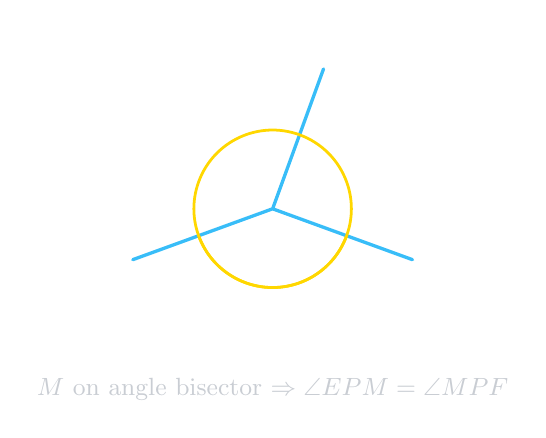
\begin{tikzpicture}[scale=0.9]
  \def\r{2.1}
  \coordinate (P) at (0,0);
  \coordinate (E) at ({\r*cos(200)},{\r*sin(200)});
  \coordinate (F) at ({\r*cos(340)},{\r*sin(340)});
  \coordinate (M) at ({\r*cos(70)},{\r*sin(70)});
  \draw[base] (P) circle (\r);
  \node[dot,label={[lab]below:$P$}] at (P) {};
  \node[dot,label={[lab]left:$E$}] at (E) {};
  \node[dot,label={[lab]right:$F$}] at (F) {};
  \node[dot,label={[lab]above:$M$}] at (M) {};
  \draw[new] (P)--(E) (P)--(F) (P)--(M);
  \pic[ang,"",lab,angle radius=10mm,angle eccentricity=1.1] {angle=E--P--M};
  \pic[ang,"",lab,angle radius=10mm,angle eccentricity=1.1] {angle=M--P--F};
  \node[labm] at (0,-2.55) {$M$ on angle bisector $\Rightarrow \angle EPM=\angle MPF$};
\end{tikzpicture}
\end{StepDiagram}

\Step{2} In triangles $\triangle PME$ and $\triangle PMF$:
\[
PE=PF \ (\text{radii}),\quad PM=PM,\quad \angle EPM=\angle MPF.
\]
So $\triangle PME \cong \triangle PMF$ (SAS).
\EqDiagram{SAS congruence $\Rightarrow ME=MF$.}

\[
\boxed{ME=MF}
\]
\end{QAPair}

% ============================================================
% Q8
\begin{QAPair}{Question 8}
\textcolor{gold}{\bfseries Question:} Two circles are centred at $A$ and $B$. $CD$ and $EF$ are chords with $CD=12$ cm, $EF=8$ cm and $\angle CAD=\angle EBF$. If radius of circle $B$ is $4$ cm, find radius of circle $A$.
\tcblower
\textcolor{green}{\bfseries Answer:}\par

\Step{1} Equal central angles $\Rightarrow$ chord length is proportional to radius:
\[
\frac{CD}{EF}=\frac{r_A}{r_B}.
\]
\begin{StepDiagram}
\begin{tikzpicture}[scale=0.9]
  \def\rA{2.2}
  \def\rB{1.4}
  \coordinate (A) at (-2.7,0);
  \coordinate (B) at ( 2.7,0);
  \draw[base] (A) circle (\rA);
  \draw[base] (B) circle (\rB);
  \node[dot,label={[lab]below:$A$}] at (A) {};
  \node[dot,label={[lab]below:$B$}] at (B) {};
  \coordinate (C) at ($(A)+({\rA*cos(20)},{\rA*sin(20)})$);
  \coordinate (D) at ($(A)+({\rA*cos(120)},{\rA*sin(120)})$);
  \coordinate (E) at ($(B)+({\rB*cos(20)},{\rB*sin(20)})$);
  \coordinate (F) at ($(B)+({\rB*cos(120)},{\rB*sin(120)})$);
  \draw[new] (C)--(D);
  \draw[new] (E)--(F);
  \draw[base] (A)--(C) (A)--(D);
  \draw[base] (B)--(E) (B)--(F);
  \pic[ang,"$\theta$",lab,angle radius=7mm,angle eccentricity=1.1] {angle=C--A--D};
  \pic[ang,"$\theta$",lab,angle radius=7mm,angle eccentricity=1.1] {angle=E--B--F};
\end{tikzpicture}
\end{StepDiagram}

\Step{2} Substitute values:
\[
\frac{12}{8}=\frac{r_A}{4}\Rightarrow r_A=4\cdot\frac{12}{8}=6.
\]
\EqDiagram{$r_A=6\text{ cm}$}

\[
\boxed{6\text{ cm}}
\]
\end{QAPair}

% ============================================================
% Q9
\begin{QAPair}{Question 9}
\textcolor{gold}{\bfseries Question:} In cyclic quadrilateral $ABDC$, $AB=CD$. Prove that $AC=BD$.
\tcblower
\textcolor{green}{\bfseries Answer:}\par

\Step{1} Equal chords subtend equal angles at the circumference:
\[
AB=CD \Rightarrow \angle ADB=\angle CAD
\quad (\text{each subtends its equal chord}).
\]
\begin{StepDiagram}
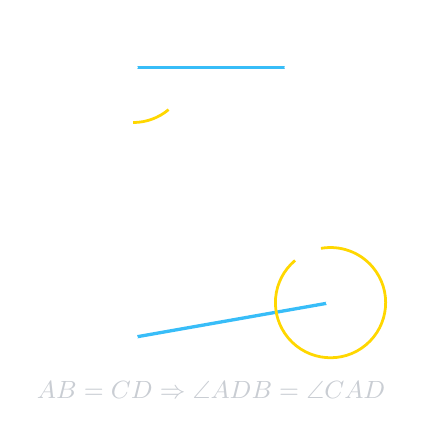
\begin{tikzpicture}[scale=0.9]
  \def\r{2.2}
  \coordinate (O) at (0,0);
  \coordinate (A) at ({\r*cos(120)},{\r*sin(120)});
  \coordinate (B) at ({\r*cos(60)},{\r*sin(60)});
  \coordinate (D) at ({\r*cos(320)},{\r*sin(320)});
  \coordinate (C) at ({\r*cos(240)},{\r*sin(240)});
  \draw[base] (O) circle (\r);
  \draw[new] (A)--(B);
  \draw[new] (C)--(D);
  \draw[base] (A)--(D);
  \draw[base] (A)--(C);
  \draw[base] (B)--(D);
  \node[dot,label={[lab]above left:$A$}] at (A) {};
  \node[dot,label={[lab]above right:$B$}] at (B) {};
  \node[dot,label={[lab]below right:$D$}] at (D) {};
  \node[dot,label={[lab]below left:$C$}] at (C) {};
  \pic[ang,"",lab,angle radius=7mm,angle eccentricity=1.15] {angle=A--D--B};
  \pic[ang,"",lab,angle radius=7mm,angle eccentricity=1.15] {angle=C--A--D};
  \node[labm] at (0,-2.65) {$AB=CD \Rightarrow \angle ADB=\angle CAD$};
\end{tikzpicture}
\end{StepDiagram}

\Step{2} Angles in the same segment (same chord $AD$):
\[
\angle ABD=\angle ACD \quad (\text{both subtend chord }AD).
\]
\EqDiagram{$\angle ABD=\angle ACD$ (same chord $AD$).}

\Step{3} Hence $\triangle ABD \sim \triangle ACD$ (AA similarity), so corresponding sides are equal:
\[
BD=AC.
\]
\begin{StepDiagram}
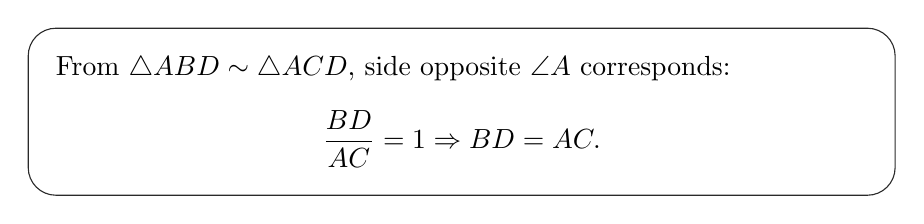
\begin{tikzpicture}[scale=0.9]
  \node[draw=border, rounded corners=10pt, inner sep=10pt, align=left, text width=0.85\linewidth]{
  From $\triangle ABD \sim \triangle ACD$, side opposite $\angle A$ corresponds:
  \[
  \frac{BD}{AC}=1 \Rightarrow BD=AC.
  \]
  };
\end{tikzpicture}
\end{StepDiagram}

\[
\boxed{AC=BD}
\]
\end{QAPair}

% ============================================================
% Q10
\begin{QAPair}{Question 10}
\textcolor{gold}{\bfseries Question:} $ABC$ is an isosceles triangle inscribed in a circle (centre $O$). Prove that $AD$ bisects $\angle BDC$.
\tcblower
\textcolor{green}{\bfseries Answer:}\par

\Step{1} Isosceles $\triangle ABC$ means $AB=AC$ (equal chords).
\begin{StepDiagram}
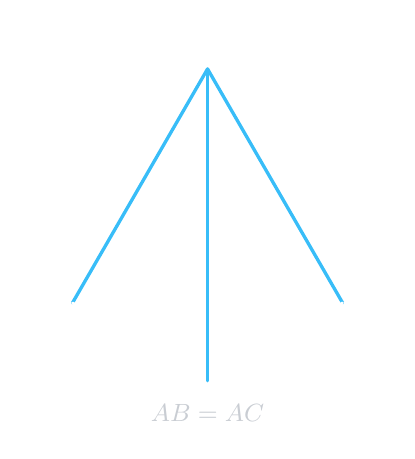
\begin{tikzpicture}[scale=0.9]
  \def\r{2.2}
  \coordinate (O) at (0,0);
  \coordinate (A) at ({\r*cos(90)},{\r*sin(90)});
  \coordinate (B) at ({\r*cos(210)},{\r*sin(210)});
  \coordinate (C) at ({\r*cos(330)},{\r*sin(330)});
  \coordinate (D) at ({\r*cos(270)},{\r*sin(270)});
  \draw[base] (O) circle (\r);
  \node[dot,label={[lab]right:$O$}] at (O) {};
  \node[dot,label={[lab]above:$A$}] at (A) {};
  \node[dot,label={[lab]left:$B$}] at (B) {};
  \node[dot,label={[lab]right:$C$}] at (C) {};
  \node[dot,label={[lab]below:$D$}] at (D) {};
  \draw[new] (A)--(B);
  \draw[new] (A)--(C);
  \draw[base] (B)--(D) (C)--(D);
  \draw[new] (A)--(D);
  \node[labm] at (0,-2.65) {$AB=AC$};
\end{tikzpicture}
\end{StepDiagram}

\Step{2} Equal chords subtend equal arcs:
\[
AB=AC \Rightarrow \widehat{AB}=\widehat{AC}.
\]
\EqDiagram{$AB=AC \Rightarrow \widehat{AB}=\widehat{AC}.$}

\Step{3} Inscribed angles at $D$ subtending equal arcs are equal:
\[
\angle BDA=\tfrac12\,\widehat{BA},\qquad \angle ADC=\tfrac12\,\widehat{AC}
\Rightarrow \angle BDA=\angle ADC.
\]
\begin{StepDiagram}
\begin{tikzpicture}[scale=0.9]
  \def\r{2.2}
  \coordinate (A) at ({\r*cos(90)},{\r*sin(90)});
  \coordinate (B) at ({\r*cos(210)},{\r*sin(210)});
  \coordinate (C) at ({\r*cos(330)},{\r*sin(330)});
  \coordinate (D) at ({\r*cos(270)},{\r*sin(270)});
  \coordinate (O) at (0,0);
  \draw[base] (O) circle (\r);
  \draw[new] (A)--(D);
  \draw[base] (D)--(B) (D)--(C);
  \node[dot,label={[lab]below:$D$}] at (D) {};
  \pic[ang,"$\alpha$",lab,angle radius=7mm,angle eccentricity=1.2] {angle=B--D--A};
  \pic[ang,"$\alpha$",lab,angle radius=7mm,angle eccentricity=1.2] {angle=A--D--C};
\end{tikzpicture}
\end{StepDiagram}

\Step{4} Therefore $AD$ bisects $\angle BDC$.
\[
\boxed{\angle BDA=\angle ADC \Rightarrow AD \text{ bisects } \angle BDC.}
\]
\end{QAPair}

% ============================================================
% Q11
\begin{QAPair}{Question 11}
\textcolor{gold}{\bfseries Question:} $ABCDE$ is a pentagon inscribed in a circle. If $AB=BC=CD$, $\angle BCD=130^\circ$ and $\angle BAE=120^\circ$, find:
(a) $\angle ABC$ \; (b) $\angle CDE$ \; (c) $\angle AED$ \; (d) $\angle EAD$.
\tcblower
\textcolor{green}{\bfseries Answer:}\par

\Step{1} Let arcs (or central angles) for equal chords be:
\[
\widehat{AB}=\widehat{BC}=\widehat{CD}=x.
\]
\begin{StepDiagram}
\begin{tikzpicture}[scale=0.92]
  \def\r{2.15}
  \coordinate (O) at (0,0);
  \coordinate (A) at ({\r*cos(170)},{\r*sin(170)});
  \coordinate (B) at ({\r*cos(220)},{\r*sin(220)});
  \coordinate (C) at ({\r*cos(270)},{\r*sin(270)});
  \coordinate (D) at ({\r*cos(320)},{\r*sin(320)});
  \coordinate (E) at ({\r*cos(110)},{\r*sin(110)});
  \draw[base] (O) circle (\r);
  \node[dot,label={[lab]right:$O$}] at (O) {};
  \foreach \P/\pos in {A/left,B/below left,C/below,D/below right,E/above}{
    \node[dot,label={[lab]\pos:$\P$}] at (\P) {};
  }
  \draw[new] (A)--(B) (B)--(C) (C)--(D);
  \draw[help] (A)--(E) (D)--(E); % just to show shape
  \node[labm] at (0,-2.7) {$AB=BC=CD \Rightarrow \widehat{AB}=\widehat{BC}=\widehat{CD}=x$};
\end{tikzpicture}
\end{StepDiagram}

\Step{2} Use $\angle BCD=130^\circ$:
\[
\angle BCD=\tfrac12\,\widehat{BD}\Rightarrow \widehat{BD}=260^\circ.
\]
But $\widehat{BD}$ (not containing $C$) is $\widehat{BA}+\widehat{AE}+\widehat{ED}=x+z+y$.
So:
\[
x+y+z=260^\circ.
\]
\EqDiagram{$\widehat{BD}=2\angle BCD=260^\circ \Rightarrow x+y+z=260^\circ.$}

\Step{3} Total circle:
\[
x+x+x+y+z=360^\circ \Rightarrow 3x+y+z=360^\circ.
\]
Subtracting with $x+y+z=260^\circ$:
\[
(3x+y+z)-(x+y+z)=360-260 \Rightarrow 2x=100 \Rightarrow x=50^\circ.
\]
\EqDiagram{$x=50^\circ$}

\Step{4} Use $\angle BAE=120^\circ$:
\[
\angle BAE=\tfrac12\,\widehat{BE}\Rightarrow \widehat{BE}=240^\circ.
\]
Now $\widehat{BE}$ (not containing $A$) is $\widehat{BC}+\widehat{CD}+\widehat{DE}=x+x+y=2x+y$.
So:
\[
2x+y=240^\circ \Rightarrow 100+y=240 \Rightarrow y=140^\circ.
\]
Then $y+z=360-3x=210^\circ \Rightarrow z=70^\circ$.
\EqDiagram{$y=140^\circ,\quad z=70^\circ$}

\Step{5} Now find required angles using ``inscribed angle = half intercepted arc'':
\begin{itemize}
\item[(a)] $\angle ABC=\tfrac12\,\widehat{AC}$, where $\widehat{AC}=\widehat{AE}+\widehat{ED}+\widehat{DC}=z+y+x=70+140+50=260$.
So $\angle ABC=130^\circ$.
\item[(b)] $\angle CDE=\tfrac12\,\widehat{CE}$, where $\widehat{CE}=\widehat{CB}+\widehat{BA}+\widehat{AE}=x+x+z=50+50+70=170$.
So $\angle CDE=85^\circ$.
\item[(c)] $\angle AED=\tfrac12\,\widehat{AD}$, where $\widehat{AD}=\widehat{AB}+\widehat{BC}+\widehat{CD}=3x=150$.
So $\angle AED=75^\circ$.
\item[(d)] $\angle EAD=\tfrac12\,\widehat{ED}=\tfrac12\,y=\tfrac12\cdot 140=70^\circ$.
\end{itemize}

\begin{StepDiagram}
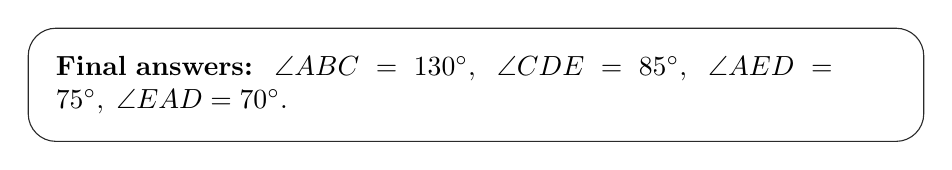
\begin{tikzpicture}[scale=0.92]
  \node[draw=border, rounded corners=10pt, inner sep=10pt, align=left, text width=0.88\linewidth]{
  \textbf{Final answers:}\;
  $\angle ABC=130^\circ,\;
  \angle CDE=85^\circ,\;
  \angle AED=75^\circ,\;
  \angle EAD=70^\circ.$};
\end{tikzpicture}
\end{StepDiagram}

\[
\boxed{\angle ABC=130^\circ,\;\angle CDE=85^\circ,\;\angle AED=75^\circ,\;\angle EAD=70^\circ}
\]
\end{QAPair}

% ============================================================
% Q12
\begin{QAPair}{Question 12}
\textcolor{gold}{\bfseries Question:} $O$ is the centre. Diameters $AB$ and $CD$ are perpendicular. Prove that joining the endpoints in order forms a square.
\tcblower
\textcolor{green}{\bfseries Answer:}\par

\Step{1} Perpendicular diameters split the circle into four equal arcs of $90^\circ$ each.
So the chords between consecutive endpoints are equal:
\[
AD=DB=BC=CA.
\]
\begin{StepDiagram}
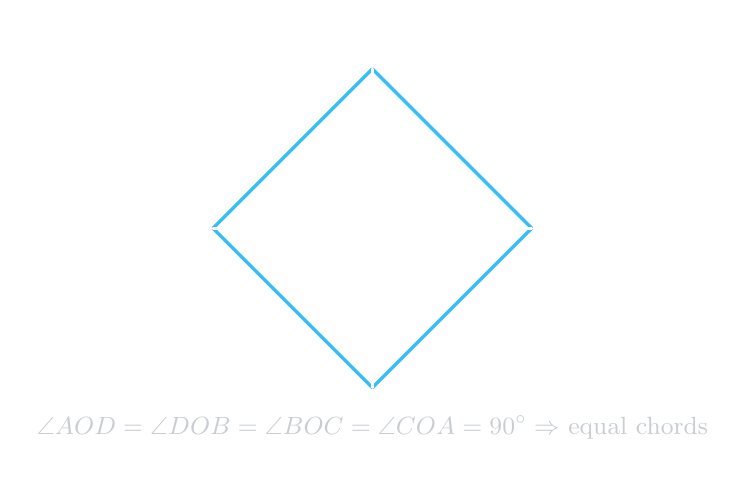
\begin{tikzpicture}[scale=0.92]
  \def\r{2.2}
  \coordinate (O) at (0,0);
  \coordinate (A) at (-\r,0);
  \coordinate (B) at ( \r,0);
  \coordinate (C) at (0,-\r);
  \coordinate (D) at (0, \r);

  \draw[base] (O) circle (\r);
  \node[dot,label={[lab]right:$O$}] at (O) {};
  \foreach \P/\pos in {A/left,B/right,C/below,D/above}{
    \node[dot,label={[lab]\pos:$\P$}] at (\P) {};
  }

  \draw[new] (D)--(B)--(C)--(A)--cycle;
  \draw[base] (A)--(B);
  \draw[base] (C)--(D);

  \node[labm] at (0,-2.75) {$\angle AOD=\angle DOB=\angle BOC=\angle COA=90^\circ \Rightarrow$ equal chords};
\end{tikzpicture}
\end{StepDiagram}

\Step{2} Since $AB$ is a diameter, the angle subtending $AB$ at $D$ is a right angle:
\[
\angle ADB=90^\circ.
\]
So the quadrilateral has all sides equal and one right angle $\Rightarrow$ it is a square.
\begin{StepDiagram}
\begin{tikzpicture}[scale=0.92]
  \def\r{2.2}
  \coordinate (A) at (-\r,0);
  \coordinate (B) at ( \r,0);
  \coordinate (D) at (0, \r);
  \coordinate (O) at (0,0);
  \draw[base] (O) circle (\r);
  \draw[new] (A)--(D)--(B);
  \draw[base] (A)--(B);
  \node[dot,label={[lab]above:$D$}] at (D) {};
  \draw[base] ($(D)+(-0.20,0)$)--($(D)+(-0.20,-0.20)$)--($(D)+(0,-0.20)$);
  \node[lab] at (0.55,1.25) {$90^\circ$};
\end{tikzpicture}
\end{StepDiagram}

\[
\boxed{\text{The endpoints joined in order form a square.}}
\]
\end{QAPair}

% ============================================================
% Q13
\begin{QAPair}{Question 13}
\textcolor{gold}{\bfseries Question:} $O$ is centre. $AB=CD$ and $\angle OAB=40^\circ$.
Find $\angle AOB$ and $\angle COD$. Are these angles equal? If yes, why?
\tcblower
\textcolor{green}{\bfseries Answer:}\par

\Step{1} In $\triangle OAB$, $OA=OB$ (radii), so base angles are equal:
\[
\angle OAB=\angle OBA=40^\circ.
\]
\begin{StepDiagram}
\begin{tikzpicture}[scale=0.92]
  \def\r{2.2}
  \coordinate (O) at (0,0);
  \coordinate (A) at ({\r*cos(150)},{\r*sin(150)});
  \coordinate (B) at ({\r*cos(40)},{\r*sin(40)});
  \draw[base] (O) circle (\r);
  \node[dot,label={[lab]below:$O$}] at (O) {};
  \node[dot,label={[lab]left:$A$}] at (A) {};
  \node[dot,label={[lab]right:$B$}] at (B) {};
  \draw[new] (O)--(A) (O)--(B) (A)--(B);
  \pic[ang,"$40^\circ$",lab,angle radius=7mm,angle eccentricity=1.18] {angle=O--A--B};
\end{tikzpicture}
\end{StepDiagram}

\Step{2} Sum of angles in $\triangle OAB$:
\[
\angle AOB=180^\circ-40^\circ-40^\circ=100^\circ.
\]
\EqDiagram{$\angle AOB=100^\circ$}

\Step{3} Equal chords subtend equal central angles:
\[
AB=CD \Rightarrow \angle AOB=\angle COD.
\]
So $\angle COD=100^\circ$ as well.
\EqDiagram{$\angle COD=100^\circ$}

\[
\boxed{\angle AOB=100^\circ,\quad \angle COD=100^\circ,\quad \text{Yes (equal chords $\Rightarrow$ equal central angles).}}
\]
\end{QAPair}

% ============================================================
% Q14
\begin{QAPair}{Question 14 (i)}
\textcolor{gold}{\bfseries Question:} Diameters $AB$ and $CD$ are perpendicular. Prove that all four chords make equal central angles.
\tcblower
\textcolor{green}{\bfseries Answer:}\par

\Step{1} Perpendicular diameters divide the circle into four $90^\circ$ central angles.
So:
\[
\angle APC=\angle CPB=\angle BPD=\angle DPA=90^\circ.
\]
\begin{StepDiagram}
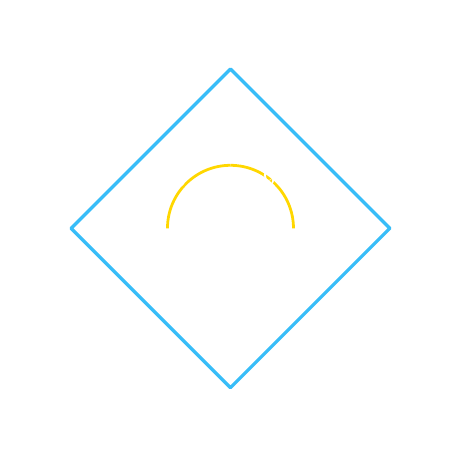
\begin{tikzpicture}[scale=0.92]
  \def\r{2.2}
  \coordinate (P) at (0,0);
  \coordinate (A) at (-\r,0);
  \coordinate (B) at ( \r,0);
  \coordinate (C) at (0, \r);
  \coordinate (D) at (0,-\r);

  \draw[base] (P) circle (\r);
  \node[dot,label={[lab]right:$P$}] at (P) {};
  \foreach \X/\pos in {A/left,B/right,C/above,D/below}{
    \node[dot,label={[lab]\pos:$\X$}] at (\X) {};
  }
  \draw[base] (A)--(B);
  \draw[base] (C)--(D);
  \draw[new] (A)--(C)--(B)--(D)--cycle;

  \pic[ang,"$90^\circ$",lab,angle radius=8mm,angle eccentricity=1.15] {angle=C--P--A};
  \pic[ang,"$90^\circ$",lab,angle radius=8mm,angle eccentricity=1.15] {angle=B--P--C};
\end{tikzpicture}
\end{StepDiagram}

\[
\boxed{\text{All four chords subtend equal central angles }(90^\circ).}
\]
\end{QAPair}

\begin{QAPair}{Question 14 (ii)}
\textcolor{gold}{\bfseries Question:} Find $\angle PCB$ and $\angle ACB$.
\tcblower
\textcolor{green}{\bfseries Answer:}\par

\Step{1} In $\triangle PCB$, $PC=PB$ (radii) and $\angle CPB=90^\circ$.
So base angles:
\[
\angle PCB=\angle PBC=\frac{180^\circ-90^\circ}{2}=45^\circ.
\]
\begin{StepDiagram}
\begin{tikzpicture}[scale=0.92]
  \def\r{2.2}
  \coordinate (P) at (0,0);
  \coordinate (B) at ( \r,0);
  \coordinate (C) at (0, \r);
  \draw[base] (P) circle (\r);
  \node[dot,label={[lab]right:$P$}] at (P) {};
  \node[dot,label={[lab]right:$B$}] at (B) {};
  \node[dot,label={[lab]above:$C$}] at (C) {};
  \draw[new] (P)--(C) (P)--(B) (C)--(B);
  \draw[base] ($(P)+(0.22,0)$)--($(P)+(0.22,0.22)$)--($(P)+(0,0.22)$);
  \node[lab] at (0.55,0.35) {$90^\circ$};
  \pic[ang,"$45^\circ$",lab,angle radius=7mm,angle eccentricity=1.2] {angle=P--C--B};
\end{tikzpicture}
\end{StepDiagram}

\Step{2} $\angle ACB$ subtends diameter $AB$, so it is a right angle:
\[
\angle ACB=90^\circ.
\]
\EqDiagram{Angle in a semicircle is $90^\circ$ $\Rightarrow \angle ACB=90^\circ$.}

\[
\boxed{\angle PCB=45^\circ,\quad \angle ACB=90^\circ}
\]
\end{QAPair}

\begin{QAPair}{Question 14 (iii)--(v)}
\textcolor{gold}{\bfseries Question:} (iii) Find other angles equal to $\angle ACB$. (iv) Name the inscribed polygon. (v) How many circles pass through the vertices?
\tcblower
\textcolor{green}{\bfseries Answer:}\par

\Step{1} Any angle subtending diameter $AB$ is $90^\circ$. So:
\[
\angle ADB=90^\circ \quad \text{(also subtends diameter }AB\text{)}.
\]
\begin{StepDiagram}
\begin{tikzpicture}[scale=0.92]
  \def\r{2.2}
  \coordinate (A) at (-\r,0);
  \coordinate (B) at ( \r,0);
  \coordinate (C) at (0, \r);
  \coordinate (D) at (0,-\r);
  \coordinate (P) at (0,0);
  \draw[base] (P) circle (\r);
  \draw[new] (A)--(D)--(B);
  \draw[base] (A)--(B);
  \node[dot,label={[lab]below:$D$}] at (D) {};
  \draw[base] ($(D)+(-0.20,0)$)--($(D)+(-0.20,0.20)$)--($(D)+(0,0.20)$);
  \node[lab] at (0.55,-1.25) {$90^\circ$};
\end{tikzpicture}
\end{StepDiagram}

\Step{2} The vertices formed (by joining $A,C,B,D$ in order) make a \textbf{square}.
\EqDiagram{Perpendicular diameters $\Rightarrow$ four equal arcs $\Rightarrow$ inscribed square.}

\Step{3} Through the vertices of a polygon (at least 3 non-collinear points), \textbf{exactly one} circle can be drawn.
\EqDiagram{A unique circle passes through any 3 non-collinear points $\Rightarrow$ only one circle through the square's vertices.}

\[
\boxed{\text{(iii) }\angle ADB;\quad \text{(iv) square;\quad (v) one circle.}}
\]
\end{QAPair}

% ============================================================
% Q15
\begin{QAPair}{Question 15}
\textcolor{gold}{\bfseries Question:} In the figure, $\widehat{RS}=3\,\widehat{PQ}$ and $\angle PTQ+\angle RTS=180^\circ$.
(i) Find $\angle PTQ$ and $\angle RTS$. (ii) Find the ratio of their measures.
\tcblower
\textcolor{green}{\bfseries Answer:}\par

\Step{1} Central angles equal the measures of their intercepted arcs (in degrees).
So:
\[
\widehat{RS}=3\,\widehat{PQ}\Rightarrow \angle RTS=3\,\angle PTQ.
\]
\begin{StepDiagram}
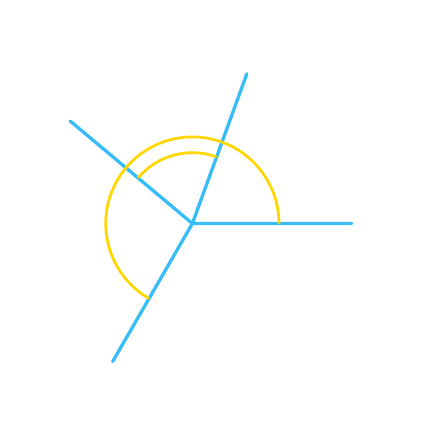
\begin{tikzpicture}[scale=0.92]
  \def\r{2.2}
  \coordinate (T) at (0,0);
  \coordinate (P) at ({\r*cos(140)},{\r*sin(140)});
  \coordinate (Q) at ({\r*cos(70)},{\r*sin(70)});
  \coordinate (S) at ({\r*cos(0)},{\r*sin(0)});
  \coordinate (R) at ({\r*cos(240)},{\r*sin(240)});
  \draw[base] (T) circle (\r);
  \node[dot,label={[lab]below:$T$}] at (T) {};
  \foreach \X/\pos in {P/above left,Q/above,S/right,R/below left}{
    \node[dot,label={[lab]\pos:$\X$}] at (\X) {};
  }
  \draw[new] (T)--(P) (T)--(Q) (T)--(R) (T)--(S);

  \pic[ang,"$x$",lab,angle radius=9mm,angle eccentricity=1.15] {angle=Q--T--P};
  \pic[ang,"$3x$",lab,angle radius=11mm,angle eccentricity=1.15] {angle=S--T--R};
\end{tikzpicture}
\end{StepDiagram}

\Step{2} Let $\angle PTQ=x$. Then $\angle RTS=3x$ and given $x+3x=180^\circ$:
\[
4x=180^\circ \Rightarrow x=45^\circ,\qquad 3x=135^\circ.
\]
\EqDiagram{$\angle PTQ=45^\circ,\quad \angle RTS=135^\circ$}

\Step{3} Ratio:
\[
\angle PTQ : \angle RTS = 45 : 135 = 1:3.
\]
\EqDiagram{Ratio $=1:3$}

\[
\boxed{\angle PTQ=45^\circ,\quad \angle RTS=135^\circ,\quad \text{ratio}=1:3}
\]
\end{QAPair}

\end{document}
